% TCGA-BRCA. Compile: pdflatex, biber, pdflatex, pdflatex.
% Template sourced from Paul's Notes, a recycled and emptied manuscript template.
% it compiles. 

% README .tex must be compiled through BIBER, to include references! 
% in tex shop select pdflatexmk, from the drop down menu!



% ============================================================
% TeXShop Compilation Guide (macOS)
% ============================================================
% 1. Place the .tex and .bib files in the same directory.
% 2. Open the .tex file in TeXShop.
% 3. Select "pdflatexmk" from the Typeset dropdown.
% 4. Click "Typeset" to compile the manuscript.
% 5. pdflatexmk automatically handles the required LaTeX
%    and Biber passes when properly configured.
%
% Citations: \parencite{reference_key}
% References: \printbibliography[title={References}]
%
% If citations fail, run the following in Terminal:
%   pdflatex manuscript.tex
%   biber manuscript
%   pdflatex manuscript.tex
%   pdflatex manuscript.tex
%
% Replace "manuscript" with the actual filename.
% ============================================================
% !TEX TS-program = pdflatexmk

%End readme.



\documentclass[12pt,letterpaper]{article}
% Image and figure support - we need this to import our images. 
\usepackage{graphicx}
\usepackage{booktabs}
\usepackage{placeins}
\usepackage{float}
\usepackage{caption}
\usepackage{booktabs}
\usepackage[T1]{fontenc}
\usepackage[utf8]{inputenc}
\usepackage{mathptmx}
\usepackage[margin=1in,headheight=15pt]{geometry}
\usepackage{setspace,fancyhdr,titlesec}
\usepackage[american]{babel}
\usepackage{csquotes}
\usepackage[backend=biber,style=apa]{biblatex}
\DeclareLanguageMapping{american}{american-apa}
%this is how we pipe in the bibliography, 
%if you use a staged .bib in git, for professional work, it go much faster then hand type.
%in git hub, place .bib into a list, then call the list. each ref is object -> pipe into call.
\addbibresource{Skeffington_Paul_TCGA_BRCA_References.bib}

% removed [hidelinks]
% We need links for TCGA compliance, to link to their website as per citation guidance. 
% Hyperlink colors: blue for URLs, citations, and internal links
\usepackage{xcolor}
\definecolor{linkblue}{HTML}{0072B2}

\usepackage[
    colorlinks=true,
    linkcolor=linkblue,
    citecolor=linkblue,
    urlcolor=linkblue
]{hyperref}

\captionsetup[table]{
    font=small,
    labelfont=bf,
    justification=raggedright,
    singlelinecheck=false,
    skip=8pt
}


\hypersetup{
  pdftitle={TCGA-BRCA: Gene Expression and PAM50 Visualization},
  pdfauthor={Paul A. Skeffington},
  pdfsubject={HSE.711 Foundations in Data Science}
}

\pagestyle{fancy}\fancyhf{}\fancyhead[R]{\thepage}\renewcommand{\headrulewidth}{0pt}
\doublespacing\raggedright\setlength{\parindent}{0.5in}\setlength{\parskip}{0pt}
\setcounter{secnumdepth}{0}
\titleformat{\section}{\normalfont\normalsize\bfseries\filcenter}{}{0pt}{}
\titlespacing{\section}{0pt}{\baselineskip}{0.5\baselineskip}
\setlength{\bibhang}{0.5in}
\newcommand{\papertitle}{TCGA-BRCA: Gene Expression and PAM50 Visualization}
\begin{document}
% cover page.
\begin{titlepage}
\thispagestyle{fancy}
\vspace*{1.6in}
\begin{center}
\textbf{\papertitle}\\[2\baselineskip]
Paul A. Skeffington\\
Master of Science in Health Data Science\\
Geisel School of Medicine at Dartmouth\\[\baselineskip]
Foundations in Data Science\\
HSE.711-FA26 \textbar{} HDOFA26\\
Instructor: Dr. Shira Fisher\\
Teaching Assistant: Erica Paulos\\[\baselineskip]
\today
\end{center}
\end{titlepage}
\setcounter{page}{2}
\begin{center}\textbf{\papertitle}\end{center}


%peroid goes after \parencite!

% ============================================================
% Introduction — POLISHED V4
% ============================================================

\section*{Introduction}

Breast cancer remains a major global public health challenge, requiring international collaboration in scientific research, clinical care, and pharmaceutical development. In 2024, approximately 2.4 million women were diagnosed with breast cancer worldwide, with an estimated 694,000 associated deaths \parencite{who2026breast}. Despite continued advances in screening and treatment, breast cancer remains a biologically heterogeneous disease, characterized by substantial variation in molecular features and clinical behavior.

Advances in gene-expression research have contributed to the identification of distinct molecular subtypes, including Luminal A, Luminal B, HER2-enriched, and Basal-like breast cancers \parencite{parker2009}. These classifications reflect differences in tumor biology and provide a framework for examining gene-expression variability across breast cancer populations. The Cancer Genome Atlas (TCGA) has further supported this research by establishing an extensive molecular resource for investigating breast cancer heterogeneity \parencite{tcga2012}.

Within this framework, two genes, ESR1 and ERBB2, were selected for their established roles in estrogen signaling and HER2-associated cellular growth pathways, respectively \parencite{tcga2012}. ESR1 (Estrogen Receptor 1) encodes estrogen receptor alpha, a transcriptional regulator involved in hormone-dependent gene expression and commonly associated with luminal breast cancer subtypes \parencite{parker2009}. ERBB2 (HER2) encodes a receptor tyrosine kinase involved in cellular growth and survival, with gene amplification or protein overexpression associated with HER2-positive breast cancer \parencite{tcga2012}.


% ============================================================
% The Data — FINAL
% ============================================================

\section*{The Data}


This research examined a gene-expression count matrix (\texttt{counts.csv}) and associated sample metadata (\texttt{meta\_data.csv}) provided through the Foundations in Data Science course (HSE.711) at the Geisel School of Medicine at Dartmouth.

The supplied files were attributed to The Cancer Genome Atlas Breast Invasive Carcinoma (TCGA-BRCA) project. Accordingly, the results presented here are based, in whole or in part, on data attributed to the \href{https://www.cancer.gov/tcga}{TCGA Research Network}. Although the files appear broadly consistent with TCGA-BRCA data, their original acquisition methods, processing procedures, and distribution history have not been independently verified. The precise relationship between the course-provided files and the original TCGA-BRCA release therefore remains subject to independent validation.

The gene-expression matrix contained measurements for 60,660 genes across 1,231 samples, accompanied by sample-level annotations. These data provided the basis for examining gene-expression distributions, recorded molecular subtype classifications, and variation among selected breast cancer-associated genes.

The TCGA research initiative was made possible through the voluntary contributions of patients who consented to the use of their biological specimens and associated clinical information for cancer research. These contributions have supported substantial advances in the genomic and molecular characterization of cancer. TCGA established informed-consent procedures and data-access safeguards to protect participants' rights while enabling scientific investigation. The continued scientific value of these contributions underscores the importance of responsible data stewardship and transparent reporting of research provenance.


% ============================================================
% METHODS — FINAL 
% ============================================================

\section*{Methods}
%Remember to use proper grammar when describing the data, data is plural, datum singular.  

Data were loaded and analyzed using R version 4.4.3 (aarch64-apple-darwin20) on macOS 26.5.2, through the RStudio development environment. Data preparation and manipulation employed the \texttt{data.table}, \texttt{dplyr}, \texttt{tibble}, and \texttt{stringr} packages. Descriptive statistics and statistical comparisons were performed using base R functions.

Visualizations were developed using \texttt{ggplot2}, with \texttt{ComplexHeatmap} and \texttt{circlize} supporting gene-expression heatmaps and standardized color mappings. Course lectures and the R Graph Gallery served as instructional resources during heatmap development. Summary tables and manuscript outputs were prepared using \texttt{knitr} and \texttt{kableExtra}. Final figures and tables were exported for incorporation into this LaTeX manuscript.

Sample identifiers were aligned by matching count-matrix column names to the metadata \texttt{barcode} field. The analysis included primary tumor, solid tissue normal, and metastatic samples. PAM50 subtype comparisons were restricted to primary tumors with classifications recorded in the \texttt{paper\_BRCA\_Subtype\_PAM50} field. Of 1,111 primary tumor samples, 1,099 had available subtype annotations; 12 were excluded from subtype-specific analyses because their classifications were missing.

For exploratory visualization, ESR1 and ERBB2 raw-count measurements were transformed using $\log_2(x+1)$ or $\log_{10}(x+1)$, depending on the graphical display. Ten breast cancer-associated genes were selected for heatmap visualization: ESR1, PGR, GATA3, FOXA1, ERBB2, GRB7, EGFR, KRT5, KRT14, and MKI67. Gene-expression measurements were standardized using row-wise Z-scores to illustrate relative expression patterns across samples. Z-score tails were used as descriptive indicators of expression variability rather than measures of statistical significance.

Descriptive statistics, including means, medians, standard deviations, and interquartile ranges, were calculated to characterize gene-expression distributions. Linear regression was used to explore the relationship between ESR1 and ERBB2 log-transformed counts.

An exploratory volcano plot compared primary tumor and solid tissue normal samples. Gene-level counts were converted to counts per million (CPM), and log2 ratios of group mean CPM values were calculated using a pseudocount of one. Welch's t-tests were used for exploratory comparisons, with resulting p-values adjusted using the Benjamini--Hochberg false-discovery-rate procedure \parencite{benjamini1995}. The volcano plot illustrated a log2 ratio threshold of $\pm 1$ and an adjusted p-value threshold of 0.05. Because this analysis did not account for sample pairing, batch effects, or RNA-seq count dispersion using a suitable count-based model, the results were interpreted as \textbf{exploratory rather than confirmatory} \parencite{love2014}.



% ============================================================
% Results - Final
% ============================================================


\section*{Results}

The dataset contained 60,660 genes across 1,231 matched samples. Of 1,111 primary tumors, 1,099 had recorded PAM50 classifications, while 12 lacked subtype annotations. Luminal A was the most prevalent subtype (571; 52.0\%), followed by Luminal B (209; 19.0\%), Basal (197; 17.9\%), HER2-enriched (82; 7.5\%), and Normal-like (40; 3.6\%). Figure~\ref{fig:pam50} and Table~1 summarize these distributions. The spiral visualization illustrates subtype proportions rather than biological relationships.

Across all samples, ESR1 exhibited a mean raw count of 31,442.2 and a median of 17,561, while ERBB2 had a mean of 46,982.5 and a median of 19,125. Both distributions were positively skewed, with higher-count observations influencing their means (Figure~\ref{fig:esr1_hist}; Table~2). ESR1 expression varied across tissue types and recorded PAM50 subtypes (Figures~\ref{fig:esr1_sample} and~\ref{fig:esr1_subtype}). Luminal B demonstrated the highest median ESR1 count (40,849), followed by Luminal A (29,436), whereas Basal (262) and HER2-enriched (652.5) exhibited the lowest medians (Table~3). These comparisons are descriptive and do not establish statistical significance.

Linear regression of log-transformed ESR1 and ERBB2 counts demonstrated a statistically significant but weak association ($R^2 = 0.017$; $p < 0.001$). The fitted relationship explained approximately 1.7\% of the observed variation in log-transformed ERBB2 counts (Figure~\ref{fig:scatter}).

A heatmap of ten selected breast cancer-associated genes illustrated relative expression patterns using row-wise Z-score standardization. Tissue-type and PAM50 annotations, together with Z-score tail summaries, provided descriptive comparisons of expression variability without implying statistical significance (Figure~\ref{fig:heatmap}).

An exploratory volcano plot compared primary tumor and solid tissue normal samples across 1,859 displayed genes (Figure~\ref{fig:volcano}). The horizontal axis represented the $\log_2$ ratio of mean counts per million (CPM), calculated with a pseudocount of one, while the vertical axis represented $-\log_{10}$ of Benjamini--Hochberg-adjusted Welch $p$-values. Illustrative thresholds were set at an absolute $\log_2$ ratio of 1 and an adjusted $p$-value of 0.05. Selected genes, including ESR1, ERBB2, EGFR, and MKI67, were labeled for interpretation. Because the analysis did not account for sample pairing, batch effects, or RNA-seq count dispersion, these observations should not be interpreted as validated differential-expression findings.



% ============================================================
% Discussion — IN PROGRESS MAJOR REVISION
% ============================================================
\section*{Discussion}

This course reinforced my existing foundations in data science while introducing new approaches to scientific visualization and reporting. I strengthened my workflows for integrating vector graphics, reference libraries, and analytical outputs into reproducible manuscripts. 

Creating my first heatmap, spiral chart, and volcano plot was particularly valuable. The spiral visualization was inspired by a presentation I attended at a neurology conference. These exercises expanded my visualization skills while highlighting the importance of accessible color palettes, particularly given my own color vision deficiency.

The course also reinforced my approach to learning through teaching. Through Paul's Notes, I document research methods and concepts to strengthen my understanding and ability to explain them. Studying breast cancer research further emphasized the contributions of patients whose donated specimens and data make this work possible.
My next research focus involves machine learning development in Rust, particularly investigating spatial variance around tumor sites. Future work will incorporate imaging and topological information to explore whether tissue structure can improve tumor boundary identification and characterization of tumor heterogeneity.


% ============================================================
% FIGURES — FIGURES WORKING NO TOUCH => CHECK [H] ON EACH .tex input!
% DO NOT USE COMPILED R .tex directly they need [H] added!
% Figures are stored in figures folder in submission .zip.
% ============================================================
\clearpage
\section*{Figures}


% Figure 1 — PAM50 subtype visualization
\begin{figure}[H]
    \centering
    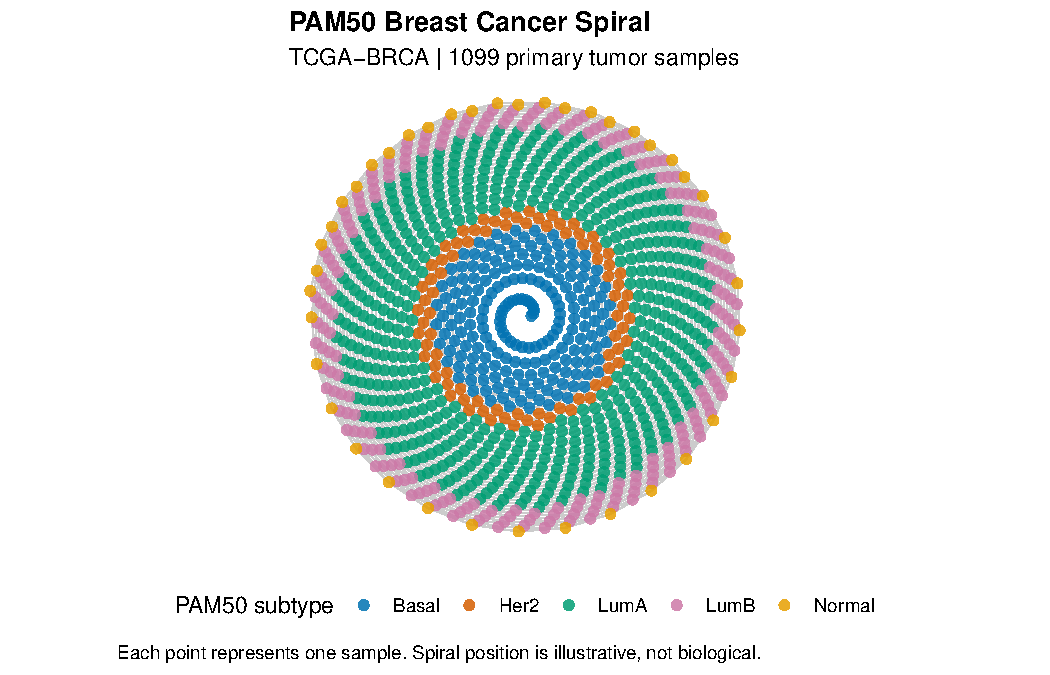
\includegraphics[width=0.85\textwidth]{figures/pam50_spiral.pdf}
    \caption{Visualization of PAM50 molecular subtypes
    in the TCGA-BRCA cohort.}
    \label{fig:pam50}
\end{figure}

% Figure 2 — ESR1 expression distribution
\begin{figure}[H]
    \centering
    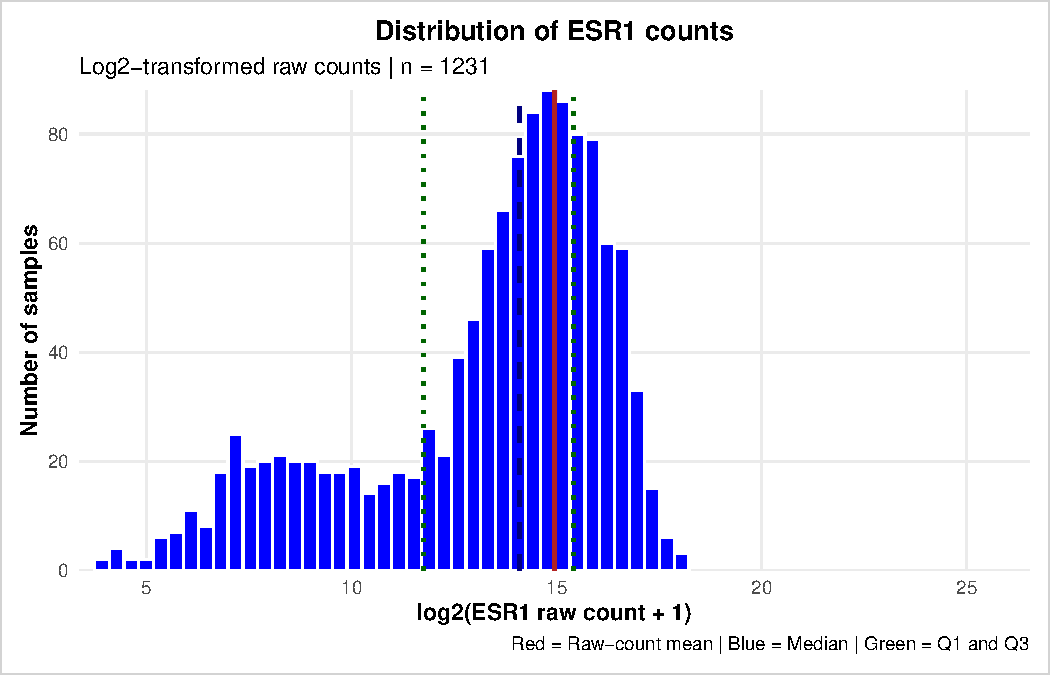
\includegraphics[width=0.85\textwidth]{figures/esr1_histogram.pdf}
    \caption{Distribution of ESR1 gene-expression values.}
    \label{fig:esr1_hist}
\end{figure}

% Figure 3 — ESR1 by sample type
\begin{figure}[H]
    \centering
    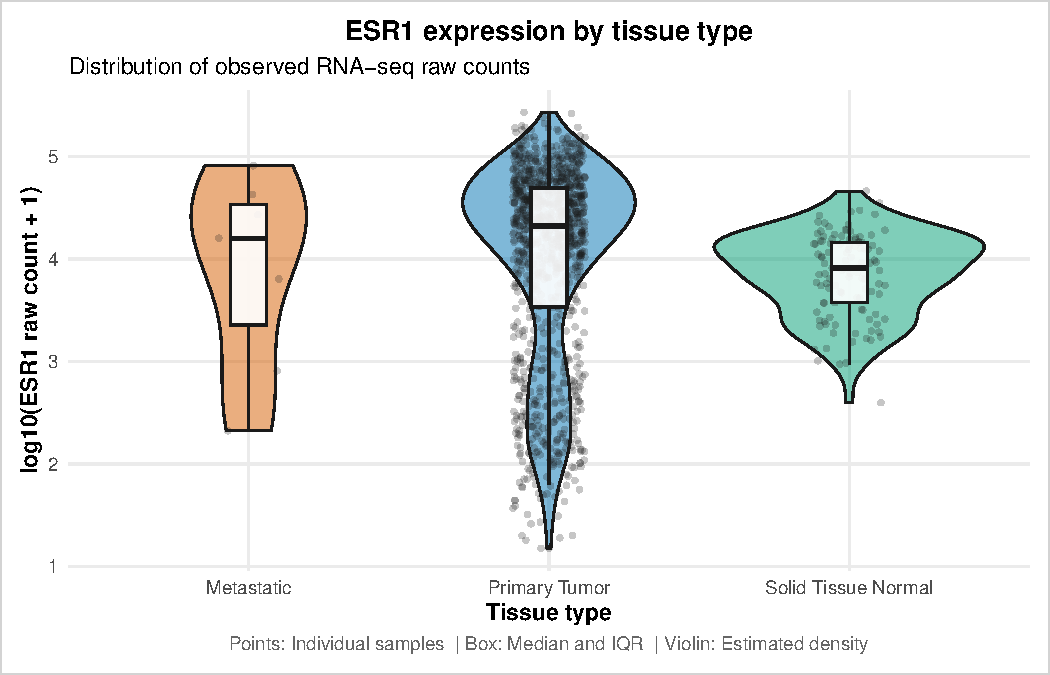
\includegraphics[width=0.85\textwidth]{figures/esr1_sample_type.pdf}
    \caption{ESR1 expression across sample types.}
    \label{fig:esr1_sample}
\end{figure}

% Figure 4 — ESR1 by PAM50 subtype
\begin{figure}[H]
    \centering
    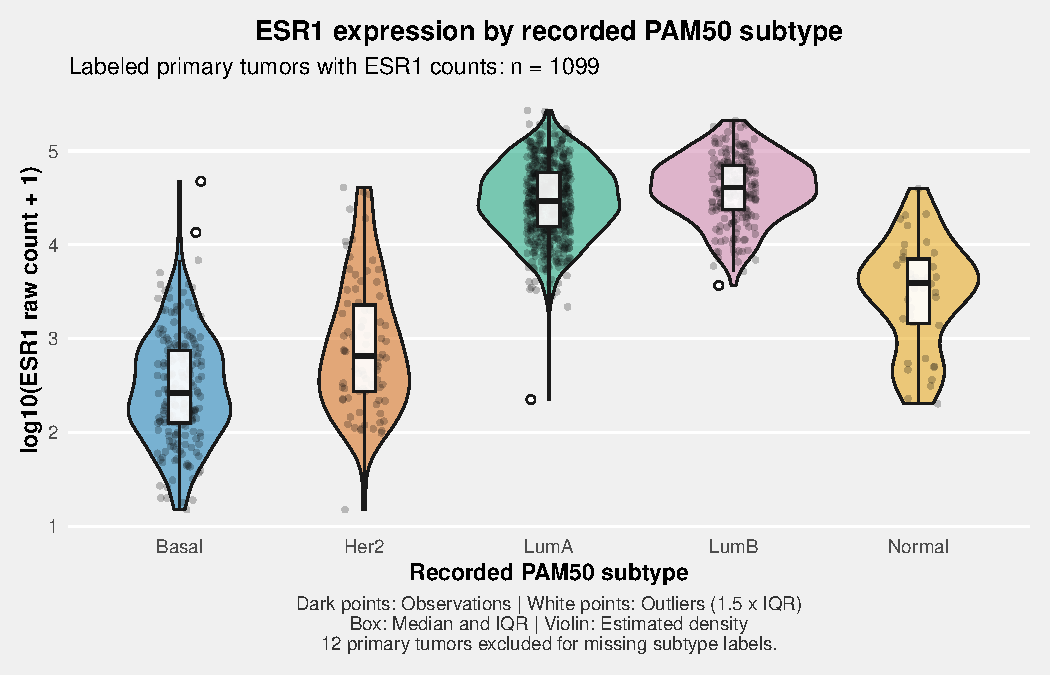
\includegraphics[width=0.85\textwidth]{figures/esr1_subtype.pdf}
    \caption{ESR1 expression across PAM50 molecular subtypes.}
    \label{fig:esr1_subtype}
\end{figure}

% Figure 5 — Gene-expression scatterplot
\begin{figure}[H]
    \centering
    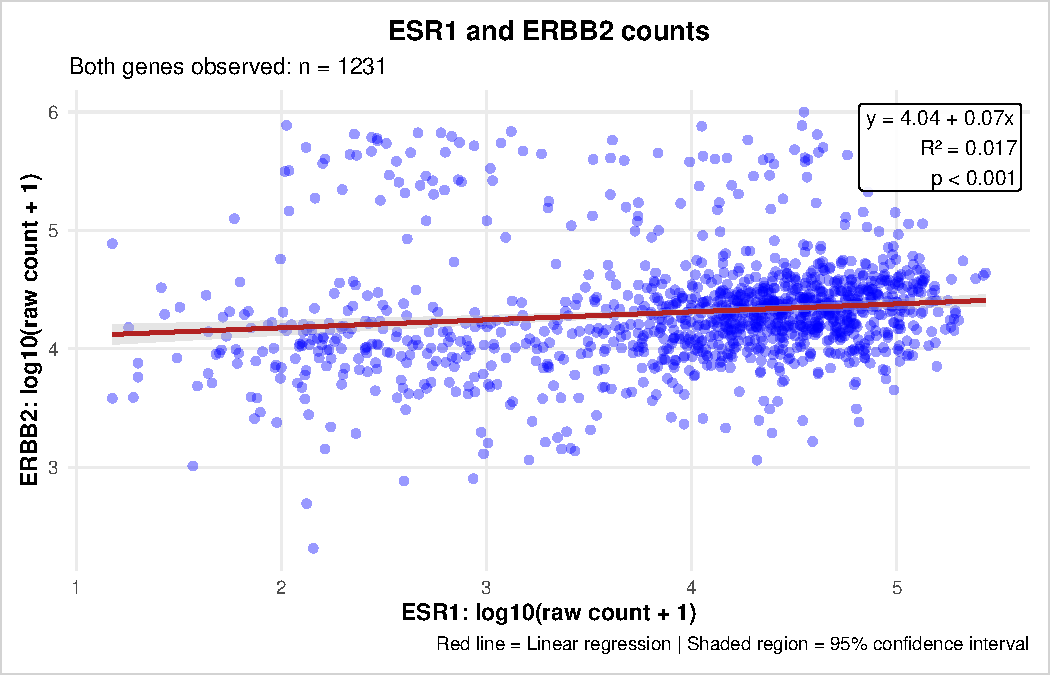
\includegraphics[width=0.85\textwidth]{figures/gene_scatter.pdf}
    \caption{Exploratory gene-expression scatterplot.}
    \label{fig:scatter}
\end{figure}

% Figure 6 — Gene-expression heatmap
\begin{figure}[H]
    \centering
    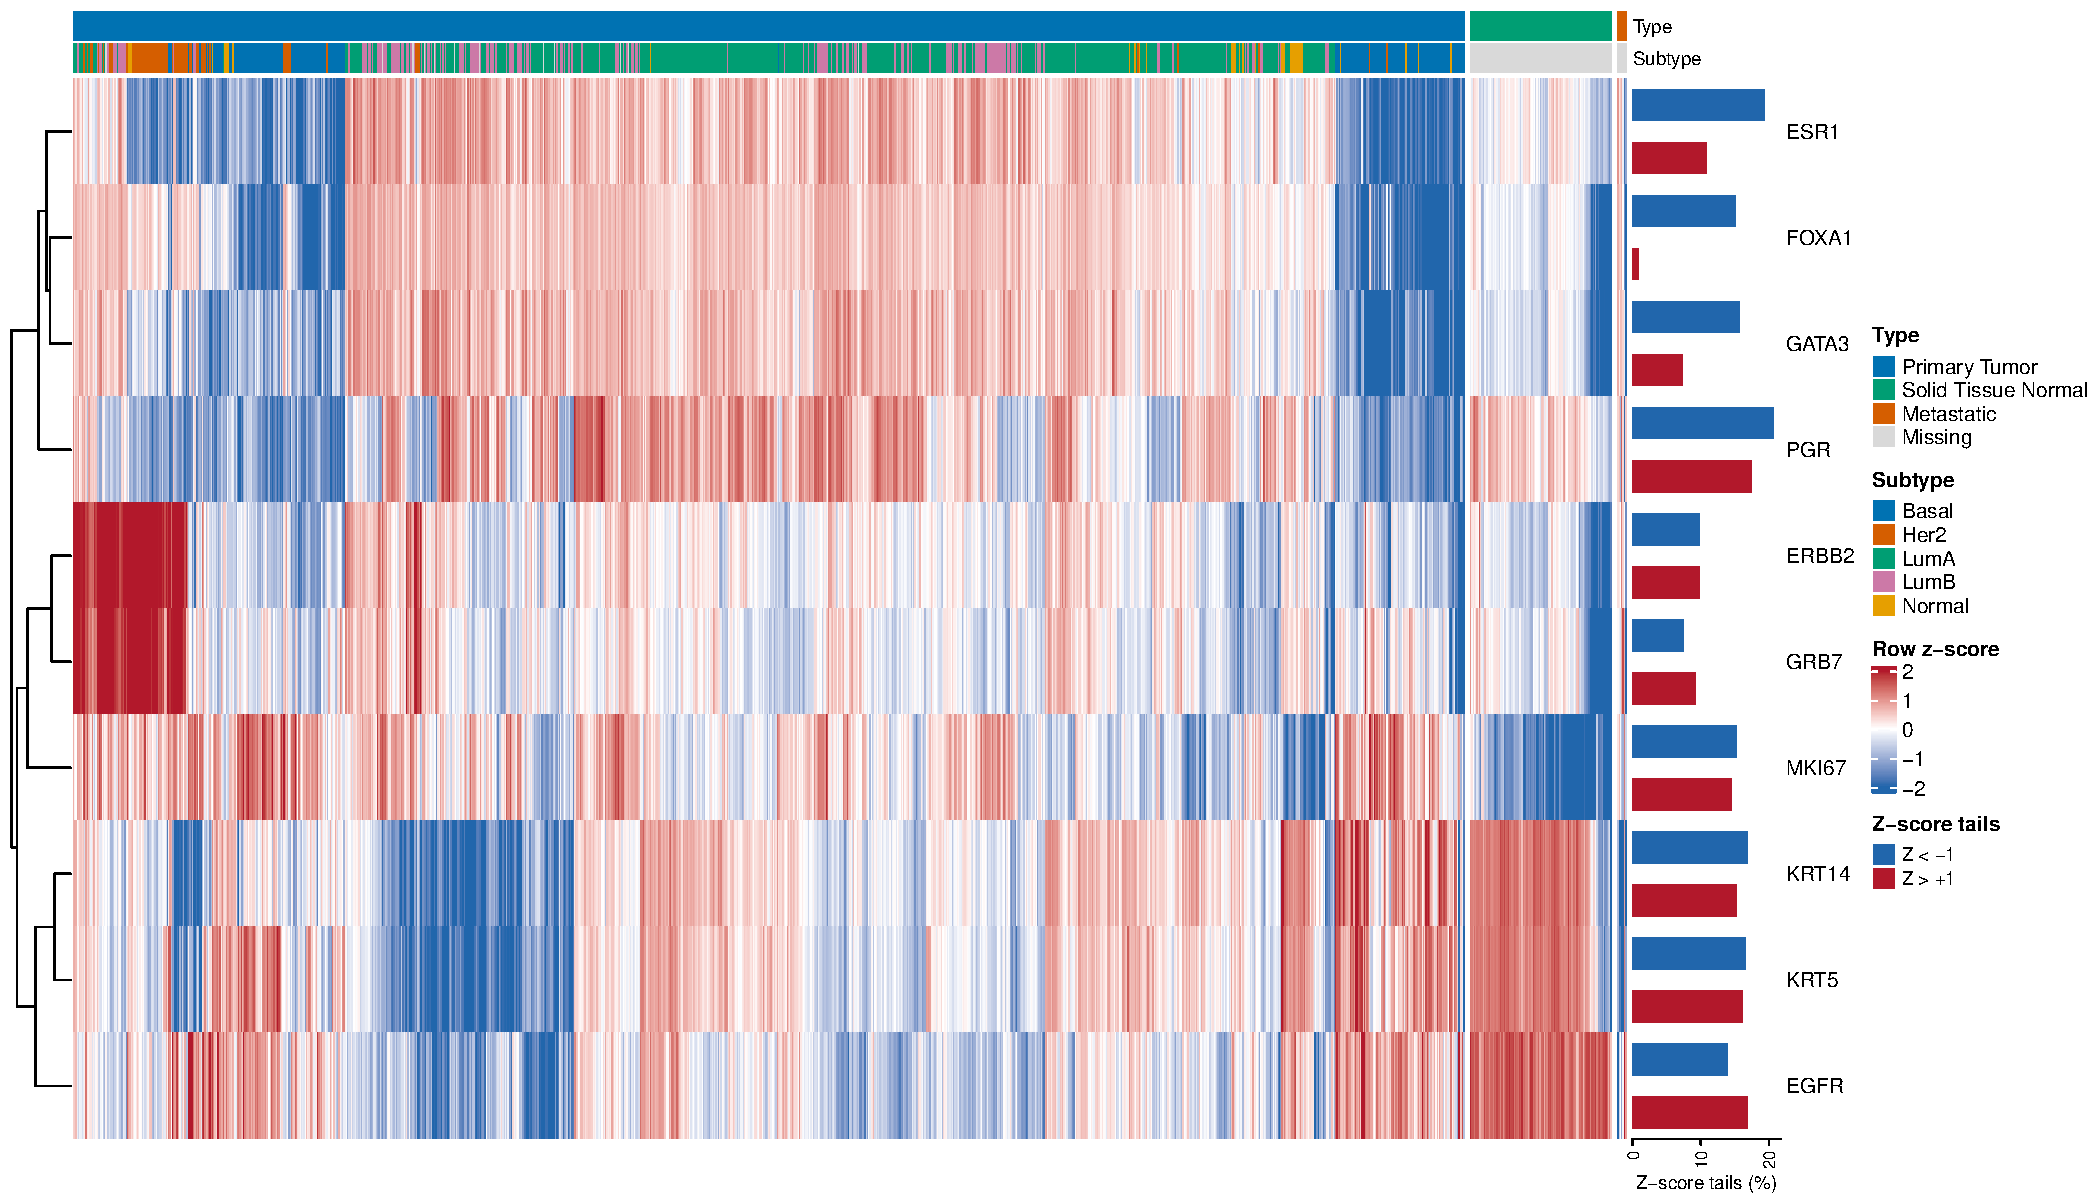
\includegraphics[width=\textwidth]{figures/gene_heatmap.pdf}
    \caption{Heatmap of selected breast cancer-associated
    gene-expression patterns.}
    \label{fig:heatmap}
\end{figure}

% Figure 7 — Exploratory volcano plot
\begin{figure}[H]
    \centering
    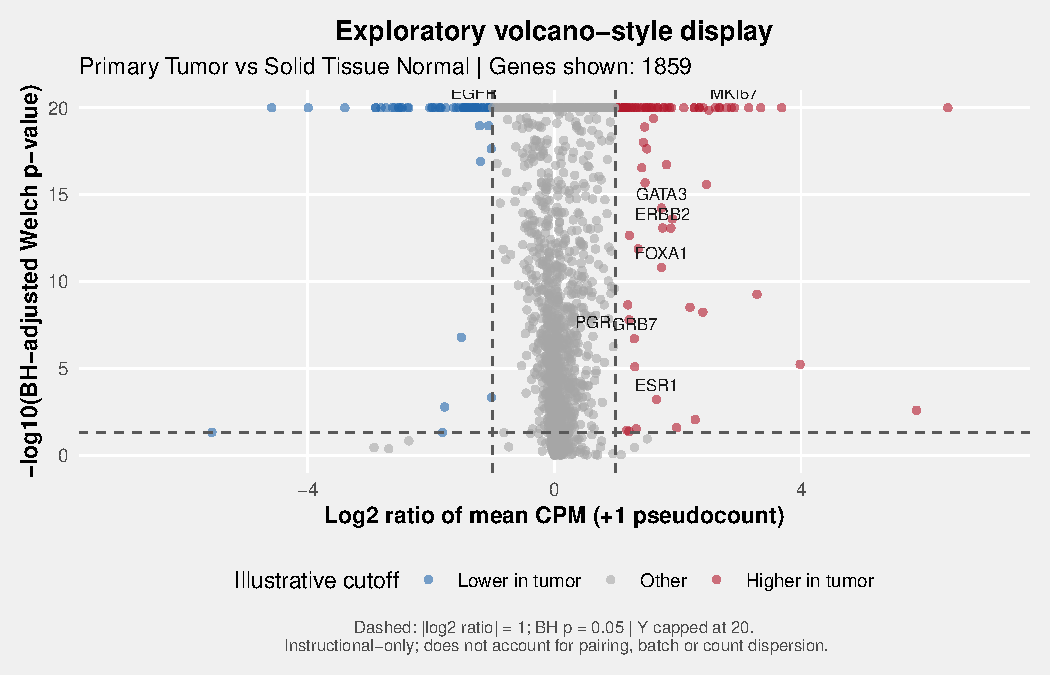
\includegraphics[width=0.85\textwidth]{figures/gene_volcano.pdf}
    \caption{Exploratory volcano plot of gene-expression
    differences between comparison groups.}
    \label{fig:volcano}
\end{figure}

% ============================================================
% TABLES WORKING NO TOUCH
% ============================================================

\clearpage
\section*{Tables}

% Table 1
\begin{table}[H]

\caption{\label{tab:export-latex-tables}PAM50 molecular subtype distribution among primary tumors.}
\centering
\begin{tabular}[t]{lrr}
\toprule
Subtype & Samples & Percent (\%)\\
\midrule
Basal & 197 & 17.9\\
Her2 & 82 & 7.5\\
LumA & 571 & 52.0\\
LumB & 209 & 19.0\\
Normal & 40 & 3.6\\
\bottomrule
\end{tabular}
\end{table}


% Table 2
\begin{table}[H]

\caption{\label{tab:export-latex-tables}ESR1 and ERBB2 raw-count descriptive statistics.}
\centering
\begin{tabular}[t]{lrrrrrrrr}
\toprule
Gene & N & Missing & Mean & Median & SD & IQR & Min & Max\\
\midrule
ESR1 & 1,231 & 0 & 31,442.2 & 17,561 & 38,261.2 & 40,242.5 & 14 & 270,977\\
ERBB2 & 1,231 & 0 & 46,982.5 & 19,125 & 105,287.5 & 19,287.0 & 205 & 995,067\\
\bottomrule
\end{tabular}
\end{table}


% Table 3
\begin{table}[H]

\caption{\label{tab:export-latex-tables}ESR1 raw-count statistics by PAM50 molecular subtype.}
\centering
\begin{tabular}[t]{lrrrrrrr}
\toprule
Subtype & N & Mean & Median & SD & IQR & Min & Max\\
\midrule
Basal & 197 & 924.5 & 262.0 & 3,589.1 & 620.0 & 14 & 47,589\\
Her2 & 82 & 3,414.2 & 652.5 & 7,745.6 & 2,010.8 & 14 & 40,971\\
LumA & 571 & 43,811.7 & 29,436.0 & 39,799.2 & 43,034.5 & 223 & 270,977\\
LumB & 209 & 53,197.4 & 40,849.0 & 41,119.8 & 46,128.0 & 3,686 & 210,656\\
Normal & 40 & 6,066.0 & 3,922.5 & 7,775.7 & 5,626.5 & 201 & 39,845\\
\bottomrule
\end{tabular}
\end{table}


\clearpage

\FloatBarrier
\clearpage

% ============================================================
% AI DISCLOSURE NO TOUCH
% ============================================================


\section*{AI Disclosure}

AI assistance was used during the initial preparation of the LaTeX manuscript template, including the removal of content from an earlier document, the creation of basic reporting placeholders, and assistance with figure file names. The manuscript was subsequently written, edited, and organized manually, with the use of additional grammar and prose-review tool disclosed below.

The following tool was used for language review and manuscript preparation:

1. \href{https://writewithharper.com/}{Harper} --- Local, non-generative grammar, spelling, and prose-style checking.

In accordance with the course AI policy, the \href{https://github.com/pskeffington/room_237}{room\_237 repository} was maintained manually. Repository operations were performed through the macOS Terminal or GitHub Desktop, while manuscript files, figures, and research outputs were edited and organized locally. The repository provides a supporting record of the project's development and document preparation.

\newpage


% ============================================================
% REFERENCES IMPORT WORKING NO TOUCH
% ============================================================

\printbibliography[title={References}]
\end{document}
